\documentclass{../exhibit}

\title{Number Mazes}

%% Font
\usepackage{imfellEnglish}
\usepackage[T1]{fontenc}
\raggedright

\usepackage{background}

\backgroundsetup{
scale=1,
color=black,
opacity=0.4,
angle=0,
contents={%
  \includegraphics[height=\paperheight]{mapBackground.jpg}%%https://upload.wikimedia.org/wikipedia/commons/8/81/Nautical_chart_of_the_West_Indies_1797.jpg
  }%
}




%% For the context
%% https://tex.stackexchange.com/questions/86150/torn-page-effect/86151#86151
\usepackage{tikz}
\usetikzlibrary{decorations.pathmorphing}
\definecolor{paper}{RGB}{239,227,157}





\renewcommand{\maketitle}{ %
  \begin{center}
    \scalebox{8}{\thetitle}
  \end{center}
  
\begin{tabular*}{\textwidth}{c @{\extracolsep{\fill}} c}  
\resizebox{4in}{!}{\begin{minipage}[b]{3in}\huge\directions\end{minipage}} &
  \resizebox{4in}{!}{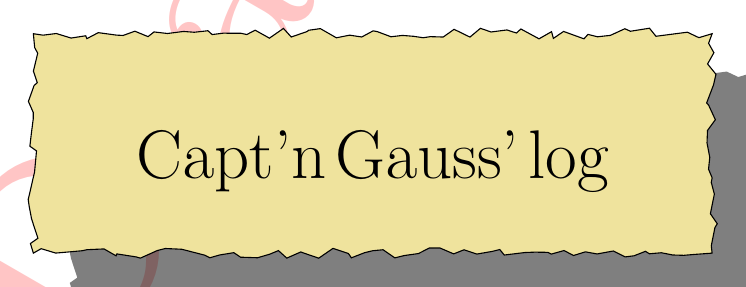
\begin{tikzpicture}[pencildraw/.style={ %
    decorate,
    decoration={random steps,segment length=4pt,amplitude=2pt}
    } %
]
\node[
preaction={fill=black,opacity=.5,transform canvas={xshift=.5cm,yshift=-.5cm}},
pencildraw,draw,fill=paper,text width=3in,inner sep=.5cm] 
{\begin{center}\Huge Capt'n Gauss' log \end{center}\vspace{.7cm} {\huge\context}};
\end{tikzpicture}}

\end{tabular*}

\vfill

\includegraphics[width=3in]{logoPirate.png}\hfill \includegraphics[width=2in]{bammLogo.png}


}


\begin{document}

\begin{context}

Land ahoy!

A treasure most fine is said to be hidden


on this mysterious island, 


by mazes of numerical design.



Unlike any seen before,


with twists and turns that defy the laws of land and sea alike.



Help me solve me maze, and learn to think in new directions!
\end{context}

\begin{directions}
  \begin{itemize}
    \item Choose a paper maze.
    \item Follow the rules of arithmetic.
    \item You cannot cross through \includegraphics[height=.5in]{skullBones.png}.
\end{itemize}
\end{directions}

\begin{example}
  \begin{center}
    Rule: Follow only increasing numbers
  \begin{tikzpicture}[scale=1.3]
    \draw[step=1.0in,black,ultra thick] (0,0) grid (4in,4in);
    \node at (0.5in,3.5in) {START};
    \node at (1.5in,3.5in) {\resizebox{!}{.8in}{3}};
    \node at (2.5in,3.5in) {\resizebox{!}{.8in}{2}};
    \node at (3.5in,3.5in) {\resizebox{!}{.8in}{3}};

    \node at (0.5in,2.5in) {\resizebox{!}{.8in}{1}};
    \node at (1.5in,2.5in) {\resizebox{!}{.8in}{2}};
    \node at (2.5in,2.5in) {\resizebox{!}{.8in}{3}};
    \node at (3.5in,2.5in) {\includegraphics[height=1in]{skullBones.png}};

    \node at (0.5in,1.5in) {\resizebox{!}{.8in}{2}};
    \node at (1.5in,1.5in) {\includegraphics[height=1in]{skullBones.png}};
    \node at (2.5in,1.5in) {\resizebox{!}{.8in}{4}};
    \node at (3.5in,1.5in) {\resizebox{!}{.8in}{3}};

    \node at (0.5in,0.5in) {\resizebox{!}{.8in}{3}};
    \node at (1.5in,0.5in) {\includegraphics[height=1in]{skullBones.png}};
    \node at (2.5in,0.5in) {\resizebox{!}{.8in}{5}};
    \node at (3.5in,0.5in) {FINISH};
    
  \end{tikzpicture}
\end{center}
\end{example}

\begin{mathConnections}
  https://bartsnapp.github.io/Math-Outreach-Exhibits/mazes/
\end{mathConnections}
\end{document}
